\tocless\section{500. Keyboard Row}
\label{algo:500}

\subsection*{Difficulty}
Easy

\subsection*{Tags}
String \& Array

\subsection*{Description}
Given a List of words, return the words that can be typed using letters of alphabet on only one row's of American keyboard like the image below.
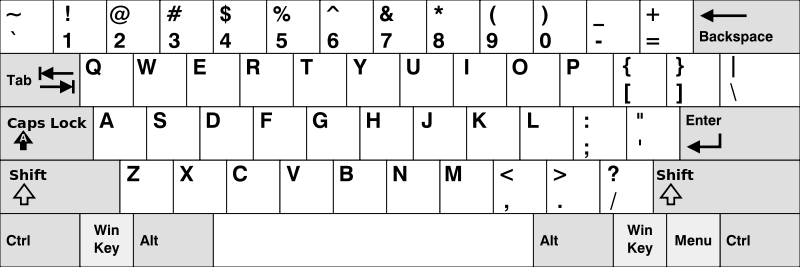
\includegraphics[width=15.8cm]{figs/algo_500_1}

\begin{example}
\begin{multilinecode}
Input: ["Hello", "Alaska", "Dad", "Peace"]
Output: ["Alaska", "Dad"]
\end{multilinecode}
\end{example}

\textbf{Note}
\begin{itemize}
    \item You may use one character in the keyboard more than once.
    \item You may assume the input string will only contain letters of alphabet.
\end{itemize}

\subsection*{Analysis}
Maybe this is a somewhat boring problem. We just need to check whether all letters of a word appear in one row of the keyboard. Therefore, we can pre-calculate the row table of the alphabet, and find in this table when iterate the words.

We assume that the number of words is $m$ and the max length of a words is $n$, then
\begin{itemize}
    \item Time Complexity: $\mathcal{O}(mn)$
    \item Space Complexity: $\mathcal{O}(1)$
\end{itemize}

\subsection*{Solution}
\subsubsection*{C}
\begin{minted}[framesep=2mm,
baselinestretch=1.2,
bgcolor=codebackground,
fontsize=\footnotesize,
linenos]{c}
char** findWords(char** words, int wordsSize, int* returnSize) {
    // row table of each letter from a to z
    int positions[] = { 1, 2, 2, 1, 0, 1, 1, 1, 0, 1, 1, 1, 2,
        2, 0, 0, 0, 0, 1, 0, 0, 2, 0, 2, 0, 2 };
    char **result = (char **)malloc(wordsSize * sizeof(char *));
    int count = 0;
    for (int i = 0; i < wordsSize; ++i) {
        char *word = words[i];
        char c = word[0];
        if (c < 'a') c += 32;  // uppercase
        int pos = positions[c - 'a'];
        for (int k = 1; (c = word[k]) != '\0'; ++k) {
            if (c < 'a') c += 32;
            // check if any letter is not in the same row as the first letter
            if (positions[c - 'a'] != pos) break;
        }
        if (c == '\0') result[count++] = word;
    }
    *returnSize = count;
    return result;
}
\end{minted}

\newpage
